\documentclass[ignorenonframetext,]{beamer}
\setbeamertemplate{caption}[numbered]
\setbeamertemplate{caption label separator}{: }
\setbeamercolor{caption name}{fg=normal text.fg}
\beamertemplatenavigationsymbolsempty
\usepackage{lmodern}
\usepackage{amssymb,amsmath}
\usepackage{ifxetex,ifluatex}
\usepackage{fixltx2e} % provides \textsubscript
\ifnum 0\ifxetex 1\fi\ifluatex 1\fi=0 % if pdftex
\usepackage[T1]{fontenc}
\usepackage[utf8]{inputenc}
\else % if luatex or xelatex
\ifxetex
\usepackage{mathspec}
\else
\usepackage{fontspec}
\fi
\defaultfontfeatures{Ligatures=TeX,Scale=MatchLowercase}
\fi
\usetheme{Warsaw}
\usefonttheme{structurebold}
% use upquote if available, for straight quotes in verbatim environments
\IfFileExists{upquote.sty}{\usepackage{upquote}}{}
% use microtype if available
\IfFileExists{microtype.sty}{%
\usepackage{microtype}
\UseMicrotypeSet[protrusion]{basicmath} % disable protrusion for tt fonts
}{}
\newif\ifbibliography
\usepackage{graphicx,grffile}
\makeatletter
\def\maxwidth{\ifdim\Gin@nat@width>\linewidth\linewidth\else\Gin@nat@width\fi}
\def\maxheight{\ifdim\Gin@nat@height>\textheight0.8\textheight\else\Gin@nat@height\fi}
\makeatother
% Scale images if necessary, so that they will not overflow the page
% margins by default, and it is still possible to overwrite the defaults
% using explicit options in \includegraphics[width, height, ...]{}
\setkeys{Gin}{width=\maxwidth,height=\maxheight,keepaspectratio}

% Prevent slide breaks in the middle of a paragraph:
\widowpenalties 1 10000
\raggedbottom

\AtBeginPart{
\let\insertpartnumber\relax
\let\partname\relax
\frame{\partpage}
}
\AtBeginSection{
\ifbibliography
\else
\let\insertsectionnumber\relax
\let\sectionname\relax
\frame{\sectionpage}
\fi
}
\AtBeginSubsection{
\let\insertsubsectionnumber\relax
\let\subsectionname\relax
\frame{\subsectionpage}
}

\setlength{\parindent}{0pt}
\setlength{\parskip}{6pt plus 2pt minus 1pt}
\setlength{\emergencystretch}{3em}  % prevent overfull lines
\providecommand{\tightlist}{%
\setlength{\itemsep}{0pt}\setlength{\parskip}{0pt}}
\setcounter{secnumdepth}{0}

\title{HHuCap: The History of Human Capital - DHB2017}
\author{Antske Fokkens, Auke Rijpma \& Richard Zijdeman}
\date{7/4/2017}

\begin{document}
\frame{\titlepage}

\begin{frame}
\tableofcontents[hideallsubsections]
\end{frame}

\begin{frame}{Quantitative approach to social mobility}

\begin{itemize}
\tightlist
\item
  usually only 2-3 observations over the life course
\item
  limited to observations, not behaviour
\end{itemize}

\end{frame}

\begin{frame}{Qualitative approach to social mobility}

\begin{itemize}
\tightlist
\item
  limited number of research persons
\item
  generally biased towards more elitish backgrounds
\end{itemize}

\end{frame}

\begin{frame}{Combining Qual and Quant}

\begin{itemize}
\tightlist
\item
  take all biographies from
  \href{http://www.biographynet.nl}{biography.net}
\item
  retrieve occupational mentions from biographies
\item
  reconstruct careers
\end{itemize}

\end{frame}

\begin{frame}{How - text wizardry}

\begin{itemize}
\tightlist
\item
  resource specific text characteristics: order, -- e.g.~first parental
  or own description
\item
  chronological information: time derived from recorded event
\end{itemize}

\end{frame}

\begin{frame}{How - social mobility part}

\begin{itemize}
\tightlist
\item
  code all occupations into a standard
\item
  apply scale scores
\end{itemize}

\end{frame}

\begin{frame}{An example: Johanna Westerdijk}

(YASGUI){[}\url{http://yasgui.org/short/B1p82-KEb}{]}
(YASGUI){[}\url{http://bit.ly/2tMwWmQ}{]}

\end{frame}

\begin{frame}{First analysis: more examples of careers}

\begin{figure}[htbp]
\centering
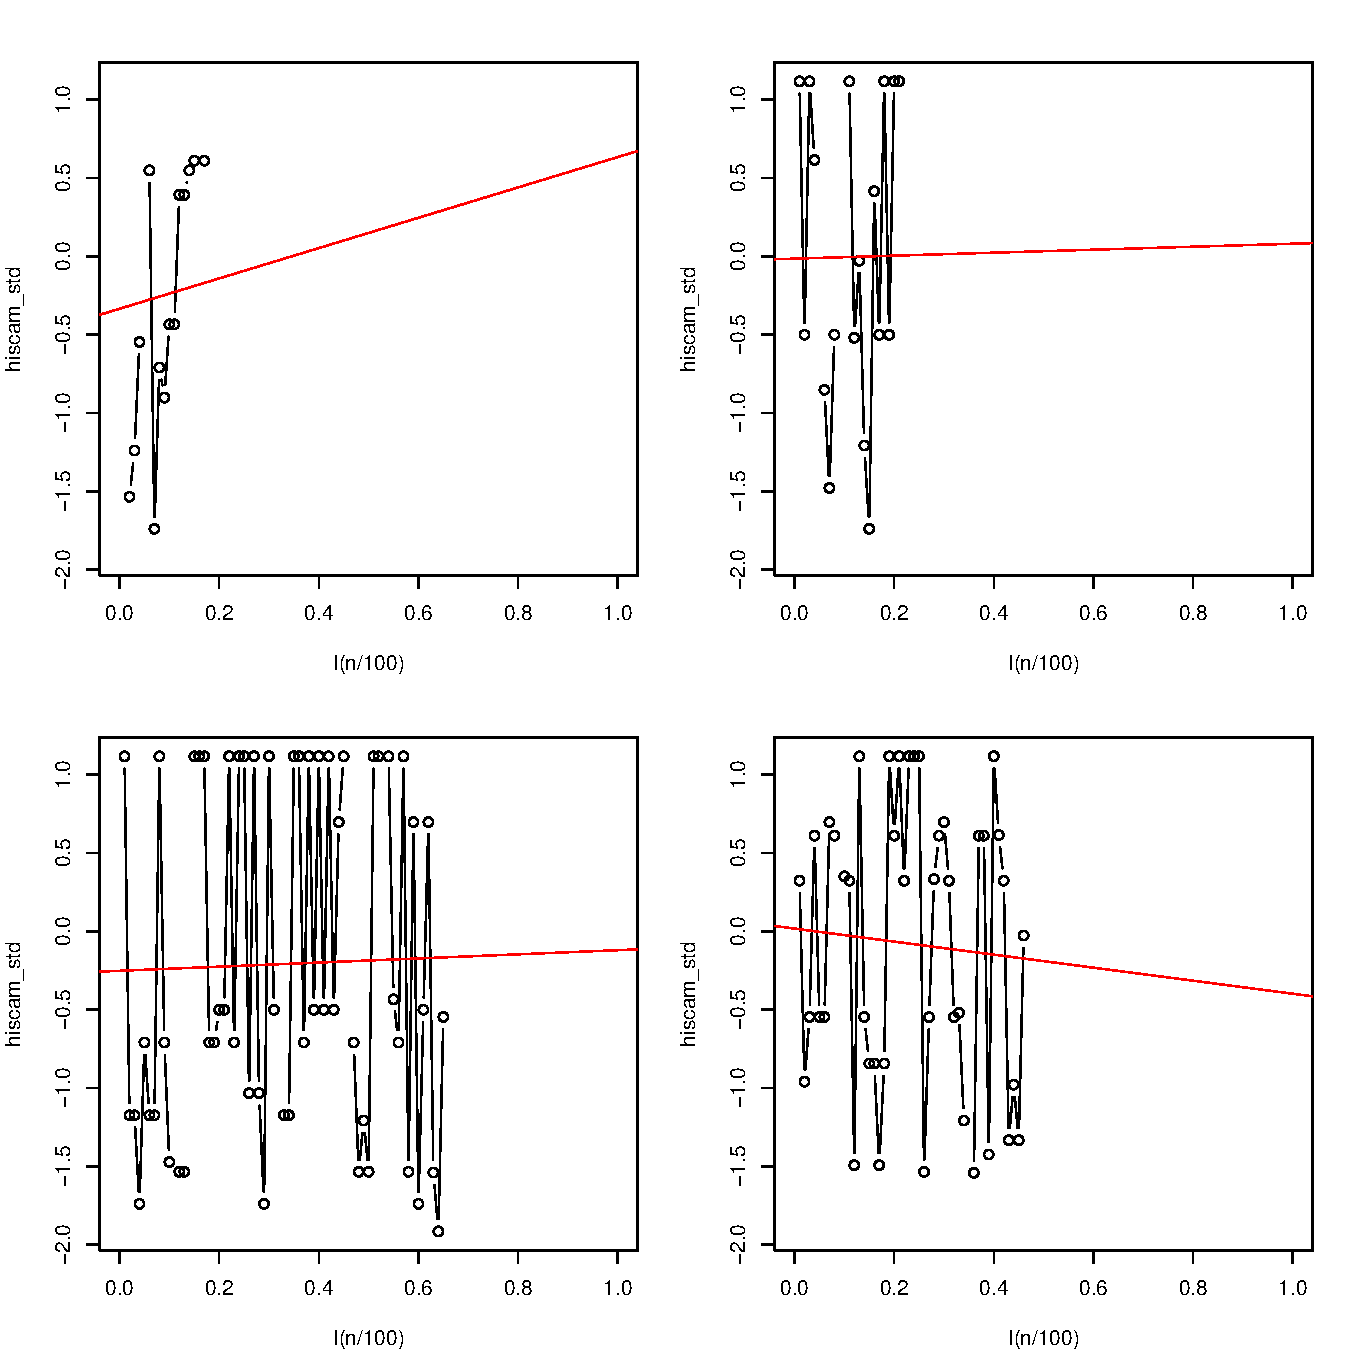
\includegraphics{../figures/careerexamples.pdf}
\caption{figure}
\end{figure}

\end{frame}

\begin{frame}{First analysis: average careers}

\begin{figure}[htbp]
\centering
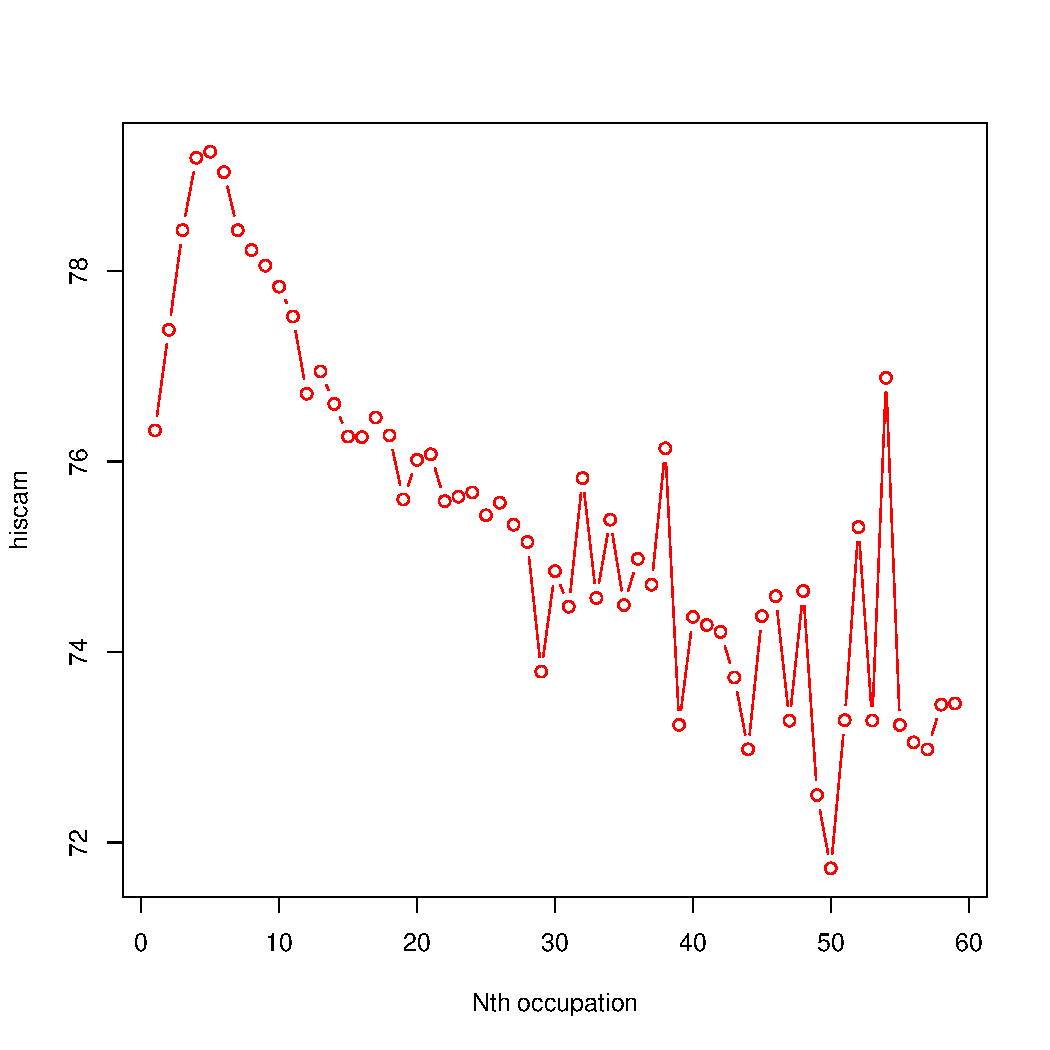
\includegraphics{../figures/avgcareers.pdf}
\caption{figure}
\end{figure}

\end{frame}

\begin{frame}{First analysis: average careers by period}

\begin{figure}[htbp]
\centering
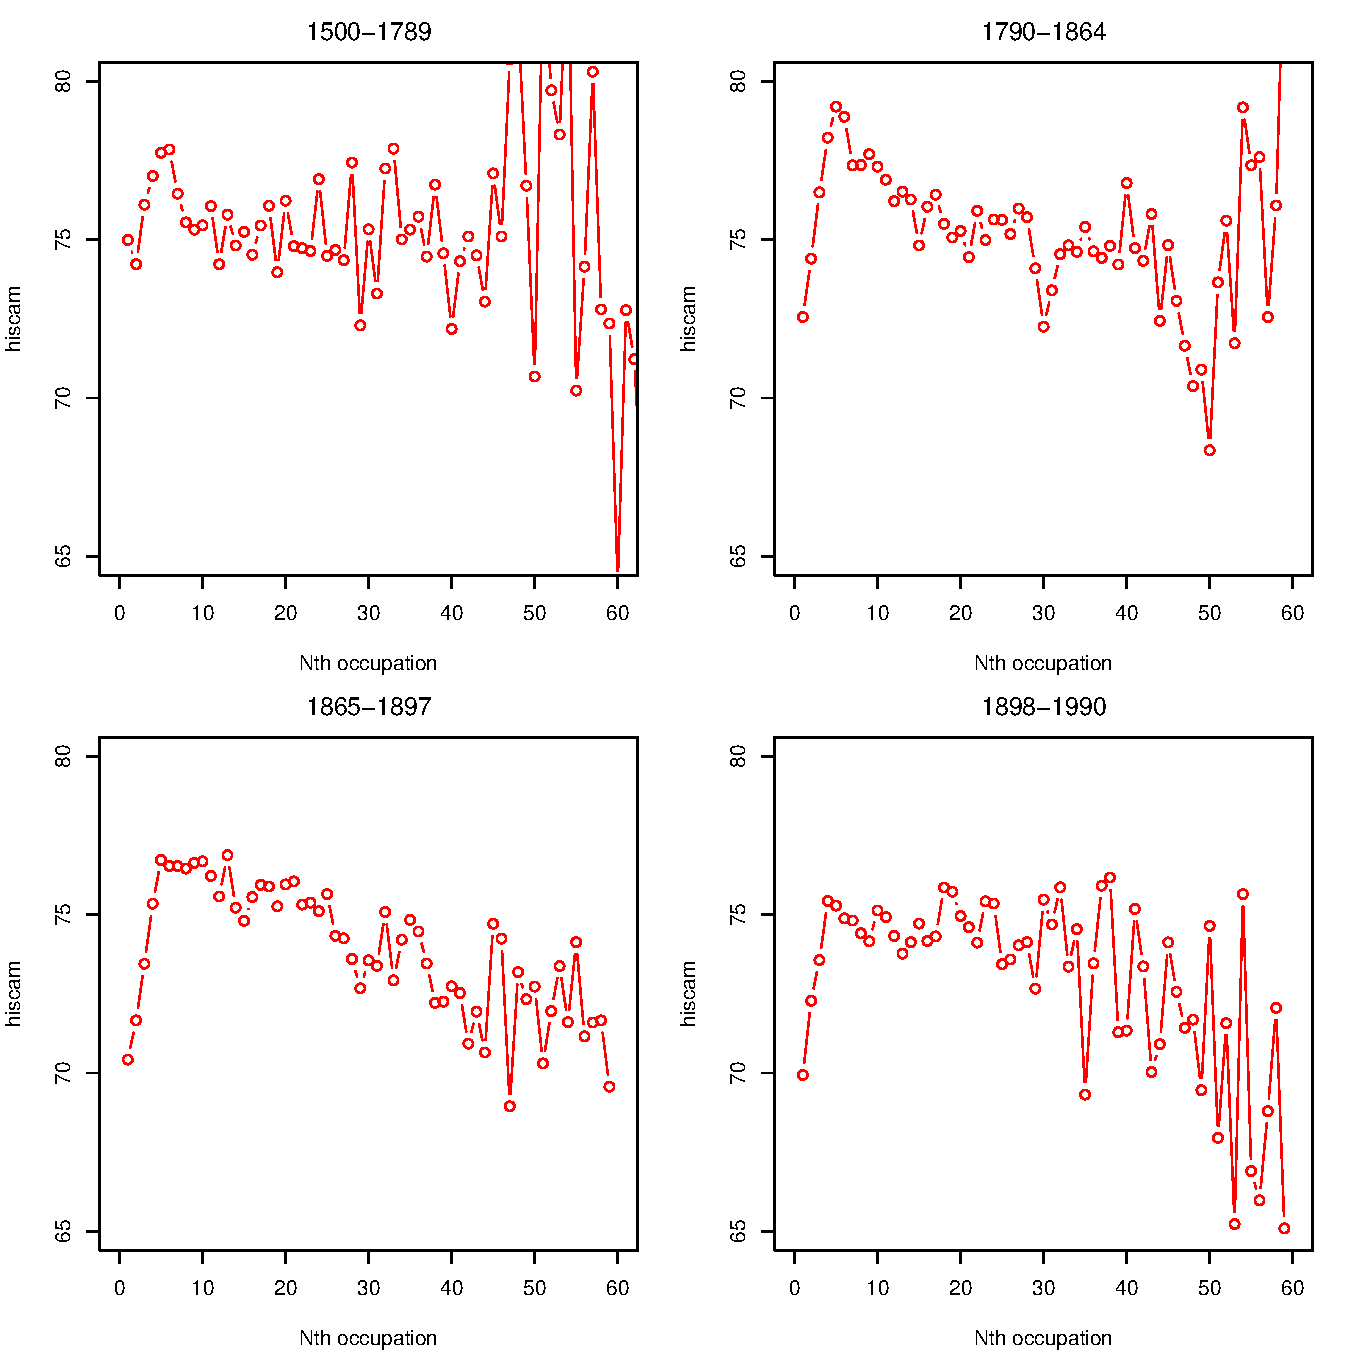
\includegraphics{../figures/avgcareers_byperiod.pdf}
\caption{figure}
\end{figure}

\end{frame}

\begin{frame}{First analysis: career growth}

\begin{figure}[htbp]
\centering
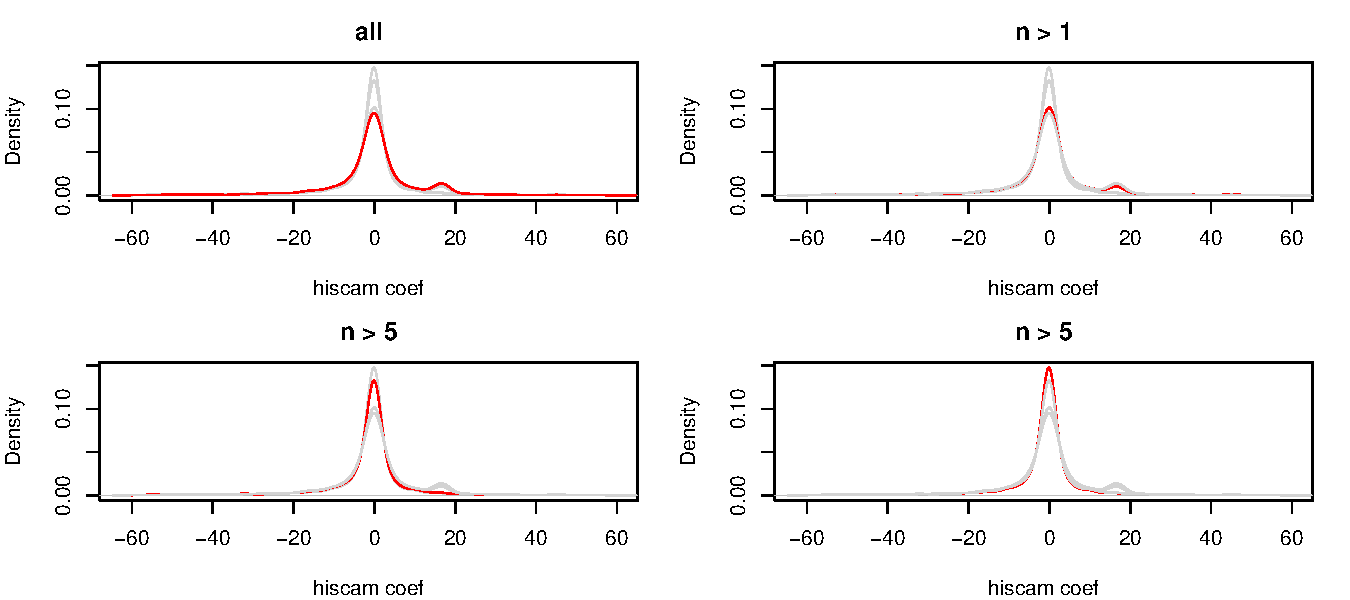
\includegraphics{../figures/careergrowth.pdf}
\caption{figure}
\end{figure}

\end{frame}

\end{document}
